\documentclass[platex,a4j,10pt,twoside,twocolumn,dvipdfmx]{jsarticle}
\usepackage[ipaex]{pxchfon} % overleaf用
%

\setlength{\textheight}{240mm}

\setlength{\textwidth}{170mm}
\setlength{\oddsidemargin}{-15mm}
\setlength{\evensidemargin}{-15mm}
\addtolength{\textwidth}{15mm}

\setlength{\textwidth}{\paperwidth}
\setlength{\oddsidemargin}{-5.4truemm}  % 左の余白を20mm(=1inch-5.4mm)に
\setlength{\evensidemargin}{-5.4truemm} % 
\addtolength{\textwidth}{-40truemm}     % 右の余白も20mmに

\setlength{\topmargin}{-15mm}
\setlength\textfloatsep{3mm}
\setlength\floatsep{2mm}

\columnsep 1.0cm
%\setlength\abovecaptionskip{-3mm} %キャプションの前に挿入されるスペース

%------------------------------------------------------------



%------------------------------------------------------------
\usepackage[dvipdfmx]{graphicx}
% \usepackage{graphicx}
\usepackage{dendentitle}
\usepackage{mediabb}
\usepackage{url}
%\usepackage[dvipdfmx]{color}
\usepackage{color}
\usepackage{amsmath,amssymb,amsopn,bm}
\usepackage{subfig}
\usepackage{multirow}
\usepackage{cite}
\usepackage{comment}
%\usepackage{natbib}
\usepackage[table,xcdraw]{xcolor}
\usepackage{float}
\usepackage{algpseudocodex, algorithm}

%------------------------------------------------------------ 関数定義
\renewcommand{\baselinestretch}{0.95}
\renewcommand{\figurename}{Fig.~}
\renewcommand{\tablename}{Table~}
\graphicspath{{./images/}}
\newcommand{\Tref}[1]{Table~\ref{#1}}
\newcommand{\Eref}[1]{式(\ref{#1})}
\newcommand{\Fref}[1]{Fig.~\ref{#1}}
\newcommand{\Sref}[1]{第\ref{#1}章}
\newcommand{\SSref}[1]{第\ref{#1}節}
\newcommand{\argmin}{\mathop{\rm arg~min}\limits}
\newcommand{\argmax}{\mathop{\rm arg~max}\limits}
\newcommand{\etal}[0]{\emph{et al}.~}

%タイトル
\title{Leveraging eBPF to Uncover the Characteristics of Shadow Attack}
\author{電子情報学専攻 修士課程2年 48-236427 手塚 尚哉}
\date{2024年5月10日}

\begin{document}
\makedendentitle{電子情報学中間報告資料}{落合研究室}
% TODO: Update the abstract with the final content. Note that this abstract is a placeholder 
% and should be updated with the final content.
% TODO: Update the abstract with the final content. Note that this abstract is a placeholder 
% and should be updated with the final content.

\section*{Abstract}
In the complex arena of cybersecurity, evasive malware,
such as shadow attacks that obscure malicious activities
through multiple processes, challenge conventional detection methods.
This paper introduces an innovative detection and analysis methodology
using Extended Berkeley Packet Filter (eBPF) technology to counteract these threats.
eBPF facilitates real-time, in-depth monitoring of system operations,
enabling the identification of sophisticated malware behaviors.

We leverage eBPF to trace process interactions and system calls,
identifying malicious patterns indicative of shadow attacks.
This approach distinguishes between legitimate and malicious activities
by analyzing process executions and network communications.
Despite challenges like data volume and behavior differentiation,
we apply smart filtering and machine learning to enhance detection accuracy.

Our research showcases eBPF's potential in detecting complex malware
through case studies, emphasizing the need for advanced analysis techniques
in cybersecurity.
This work contributes significantly to understanding and mitigating advanced malware threats,
proving eBPF as a vital tool in modern cybersecurity defenses.


\section{Introduction}
In the contemporary digital landscape, the sophistication of malware,
particularly in its ability to evade detection and analysis,
poses a significant challenge to cybersecurity efforts.
Among these evasive tactics, shadow attacks~\cite{Weiqin:ShadowAttack},
which cleverly distribute malicious activities across multiple processes,
stand out as particularly insidious.
These attacks exploit the inherent complexity of operating systems,
mimicking benign multi-process behavior to obfuscate their malicious intent.
Traditional detection mechanisms, reliant on static and dynamic analysis techniques,
often fall short in identifying these distributed threats,
necessitating the exploration of more advanced methodologies.

This paper introduces an innovative approach to tackling the
challenge posed by shadow attacks through the use of Extended Berkeley Packet Filter (eBPF).
eBPF, a technology that allows for the safe execution of custom code within the
Linux kernel without changing kernel source code or loading kernel modules,
offers a powerful mechanism for monitoring and tracing system-level operations.
Our research leverages eBPF to analyze the interconnections between function calls,
thereby revealing the execution patterns of processes involved in shadow attacks.
By mapping these patterns, we aim to uncover the stealthy operations of evasive malware,
providing insights that could lead to more effective detection and mitigation strategies.

We focus on the potential of eBPF to provide granular visibility into the behavior
of systems at runtime, enabling the identification of the complex orchestration of
processes characteristic of shadow attacks. Through the detailed analysis of function
call chains, we can trace the flow of execution within malicious processes,
identifying their strategies and mechanisms. This approach not only enhances
our understanding of how such attacks are constructed and executed but also opens
new avenues for developing countermeasures that can detect and neutralize these threats more efficiently.

By employing eBPF to dissect the intricacies of process execution and interaction in the
context of shadow attacks, we believe our research will contribute a novel perspective to the field of
cybersecurity. We demonstrate how eBPF's capabilities can be harnessed to advance our
understanding of malicious process execution, offering a promising methodology for combatting
evasive malware. Through this work, we aim to bolster the cybersecurity community's arsenal against
the ever-evolving landscape of malware threats, ensuring a more secure digital environment for all users.

Our exploration into the use of eBPF against shadow attacks not only highlights the adaptability and
complexity of modern malware but also underscores the necessity for innovative detection and analysis
techniques. As we delve into the capabilities and applications of eBPF, we pave the way for future
research and development in the domain of cybersecurity, seeking to establish more sophisticated defenses
against the cunning and elusive nature of malware attacks.


\section{Background}
\subsection{Shadow Attack \cite{Weiqin:ShadowAttack}}
Shadow Attack is one of the techniques used by malware writers to evade behavior-based detection systems,
orchestrating multiple processes to stealthily carry out malicious activities.

Such detectors typically rely on comparing system call graph within a process under scrutiny with predefined
malware specifications established on specific sequences or graphs of system calls\cite{inproceedings}.
For example, the malware specification of download-and-execute is expressed as follows \cite{Weiqin:ShadowAttack}:
\begin{equation}
  \texttt{recv} \land \texttt{open} \rightarrow \texttt{write} \rightarrow \texttt{exec}
\end{equation}
, where $s_1 \land s_2$ denotes both of two system calls $s_1, s_2$ are executed and $s_1 \rightarrow s_2$
denotes $s_1$ is followed by $s_2$.

So more specifically, the goal of Shadow Attack is to bypass dynamic malware detection based on
the analysis of system call graphs by exporting any critical system call included in malware specifications to
other collaborating processes, which is called shadow processes.
We call the Communication shadow processes do with each other as Shadow Process Communication (SPC).
The concept of Shadow Attack is illustrated in \Fref{img:shadow-attack}.
\begin{figure}[tp]
  \begin{center}
    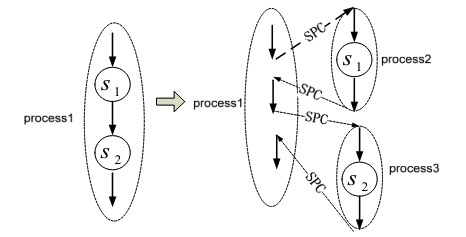
\includegraphics[width=\columnwidth]{./img/archi_SA.png}
  \end{center}
  \caption{Illustration of Shadow Attacks
    \cite{Weiqin:ShadowAttack}}
  \label{img:shadow-attack}
\end{figure}

Shadow attacks can be categorized into in-host, remote-network-coordinated, and hybrid.
In in-host shadow attacks, all shadow processes are executed on the same host and SPCs are conducted through
unix domain socket or stream pipe, while remote-network-coordinated shadow attacks involve multiple remote hosts
that are connected through network sockets.
Prototype implementation is made by the authors only for in-host shadow attacks.

One countermeasure is extracting correlation between processes and reconstructing
the original system call graph, but the authors conducted an evaluation experiment following this approach,
whose result suggested that solution would encounter challenges of high overhead.

\subsection{eBPF}
\subsubsection{Berkeley Packet Filter}
Steven and Van \cite{mccanne1993bsd} proposed the BSD Packet Filter architecture in 1993 for efficient packet capture on
Unix-based operating systems. In the following, we refer to Berkeley Packet Filter as "BPF."
At the time of paper publication, packet capture involved copying all packets acquired in the kernel
space to the user space before filtering.
This process resulted in unnecessary overhead. \cite{mccanne1993bsd} devised a pseudo-machine (BPF pseudo-machine)
that interprets programs written in special 32-bit instructions to perform filtering.
By running this pseudo-machine in the kernel space, they addressed the issue. Compared to existing systems,
BPF operated up to 20 times faster.
The overview of BPF architecture is shown in Figure \ref{img:bpf_old}.

BPF was introduced in the Linux kernel as "Linux Socket Filter" in version 2.1.75 and
was used to accelerate the \texttt{tcpdump} command.

\subsubsection{Extended Berkeley Packet Filter}
BPF underwent significant improvements and extensions in the Linux kernel version 3.18,
leading to the emergence of extended BPF, commonly referred to as eBPF \cite{Linux31836:online}.
The enhancements cover various aspects, with notable additions summarized below \cite{learning-ebpf}:
\begin{itemize}
  \item 64-Bit BPF Instruction Set: The BPF instruction set was reworked from 32-bit to 64-bit, resulting in improved execution efficiency.
  \item eBPF Maps: The introduction of eBPF maps allowed data sharing between user space and kernel space. These maps serve as a mechanism for efficient communication.
  \item eBPF Verifier: To ensure safe execution of eBPF programs, an eBPF verifier was added. It validates the correctness and security of eBPF code.
\end{itemize}

\begin{figure}[tp]
  \begin{center}
    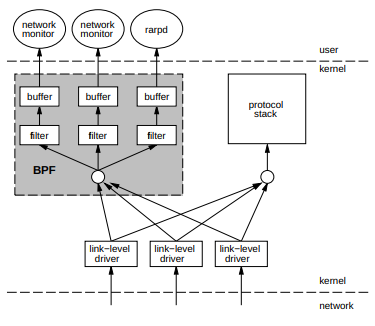
\includegraphics[width=\columnwidth]{./img/bpf_overview.png}
  \end{center}
  \caption{The overview of BPF architecture. It accelerates packet capture
    by performing filtering in the kernel space. \cite{mccanne1993bsd}}
  \label{img:bpf_old}
\end{figure}

The area covered by eBPF has also expanded.
In the context of networking, it has become able to handle various layers of the Linux network stack,
such as unix domain sockets and network devices.
Additionally, eBPF programs can now be used for performance tracing and enhancing the security of Linux systems,
leading to the term "BPF" losing its original meaning of "Berkeley Packet Filter" and being used as an independent term.

For convenience, BPF before the extension in v3.18 is sometimes referred to as classical BPF or cBPF.

\subsubsection{Overview of eBPF Architecture}
An overview of the eBPF architecture is shown in \Fref{img:ebpf-system}.
Hereafter, we describe the important processing flows with reference to \Fref{img:ebpf-system}.
\begin{figure}[tp]
  \begin{center}
    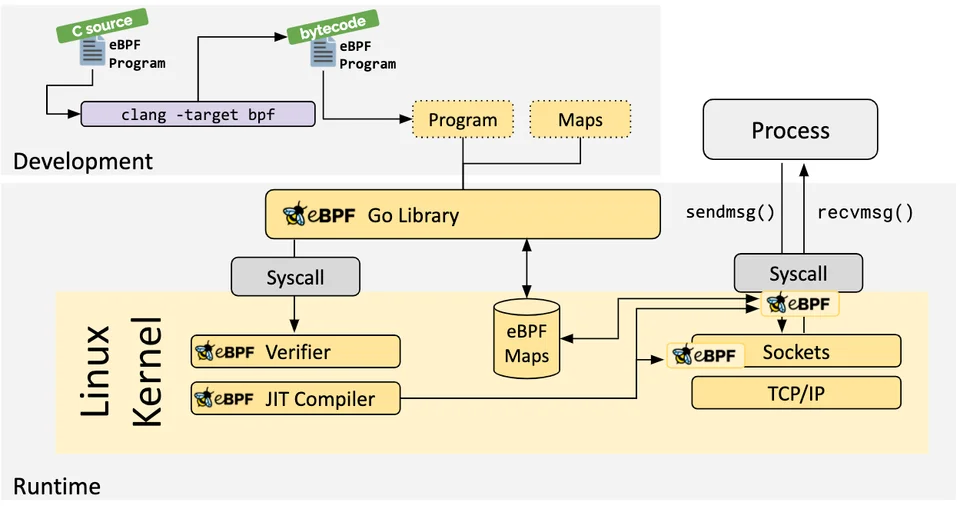
\includegraphics[width=\columnwidth]{./img/ebpf_system.png}
  \end{center}
  \caption{The overview of eBPF architecture. This figure shows how eBPF programs are compiled, verified, and executed.
    \cite{WhatiseB29:online}}
  \label{img:ebpf-system}
\end{figure}

\subsubsection{Event-Driven Architecture}

eBPF has an event-driven architecture.
The mechanism involves hooking an eBPF program to an event in the kernel, and then
performing the specified processing when the event occurs. eBPF programs can be dynamically loaded or removed.

The events that eBPF can hook into are defined as Program Types in the kernel's source code \footnote{\texttt{include/uapi/linux/bpf.h}}.
A few examples of Program Types are as follows:
\begin{itemize}
  \item XDP: An event for manipulating packets before data is copied to the kernel space when a packet arrives at a network device.
  \item Tracing: An event for detecting kernel function calls and passing tracepoints.
  \item LSM: An event for applying security policies using the Linux Security Module.
\end{itemize}
When such events occur, the eBPF program executes the processing corresponding to the Program Type.
For example, a program hooked to an XDP event can decide whether to accept or drop a packet.

\subsubsection{eBPF Verifier}
The eBPF verifier is a program that takes eBPF programs converted to bytecode as input and
verifies that they can be executed safely on the kernel.
The bytecode is loaded into the kernel via the \texttt{bpf()} system call
(shown as "Syscall" in \Fref{img:ebpf-system}), but the program will not run unless it passes verification by the verifier.
Specifically, it checks for things like avoiding memory access violations, ensuring the program exits normally,
and that the program is not granted unnecessary privileges.

In this way, the eBPF verifier enhances security by imposing restrictions on eBPF programs.
Since the verifier plays a crucial role in eBPF,
research has been conducted to mathematically verify the logic of the verifier \cite{vishwanathan2023verifying}.

\subsubsection{JIT Compilation}
The eBPF bytecode that passes the verifier is converted by a JIT compiler into machine code
that directly runs on the target CPU. This optimizes the execution speed, allowing it
to operate as efficiently as the kernel and kernel modules directly compiled from source code
\cite{WhatiseB29:online}.


\section{Related Work}
\subsection{Malware Analysis}
Malware analysis is a critical aspect of cybersecurity, enabling the identification
and mitigation of malicious software threats.
Analysis techniques can be roughly categorized into two classes: static and dynamic.

\subsubsection{Static Analysis}
Static analysis involves examining the structure and content of a suspected malicious file without executing it.
Static analysis are often conducted as a preliminary step to grasp the general characteristics of the malware
before more sophisticated analysis techniques are applied \cite{chakkaravarthy2019survey}.

\textbf{Signature matching} is a common technique that compares the "signature", characteristics of a file
against a database of malware such as VirusTotal \cite{VirusTot28:online}. The characteristics include file size, hash values, and byte sequences.
Although this method has been a staple in malware detection, it is limited by its inability to detect only known malware.

\textbf{Disassemble and decompile} is another static analysis technique
that involves converting the binary code of a malware into a human-readable format.
From the decompiled code, analysts might be able to identify the malware's functionality and behavior as well as finding
interesting strings like URLs, IP addresses, and encryption keys.

\subsubsection{Dynamic Analysis \cite{10.1145/3329786}}
Dynamic analysis entails examining the behavior of malware by executing it in a controlled environment.
This approach enables analysts to witness the interactions between the malware and the system,
providing insights into its true intentions and capabilities.

\textbf{Function call analysis} is a method that focuses on tracking functions issued by the malware and the parameters
passed to them. One way to archive this is by code injection, in which analyzing code is hooked into
a specific function call and various information is collected and notified when the function is called.
Carsten et al. \cite{willems2007toward} created an automated malware analysis system that injects DLLs within CWSandbox,
letting analysts monitor system calls.

\textbf{Data flow tracking} is another approach that tracks the flow of data through the malware, and data tainting is an established
technique in this area. It involves marking (or "tainting") specific data components and then monitoring
how this tainted data propagates through the system.
Data tainting could be utilized in static analysis, but due to some evasion strategies like encryption and obfuscation
it has endured challenges in practice \cite{alashjee2019dynamic}.
SELECTIVETAINT \cite{chen2021selectivetaint} was invented to address performance overhead issue by employing static binary
rewriting to selectively instrument only instructions related to taint analysis.

\subsection{Kernel Modules}
Kernel modules are a mechanism that allows for the extension of kernel functions without modifying the kernel's
source code by loading object files during the execution of the Linux kernel.
Kernel modules are not subject to constraints like the eBPF verifier, thus offering a high degree of program freedom.
However, since kernel modules are executed with the same privileges as the kernel,
it is necessary to develop carefully to avoid embedding vulnerabilities \cite{chen2011linux}.

As Mayer et al. \cite{mayer2021performance} point out, avoiding the creation of kernel modules can be
considered an advantage of eBPF.


\section{Proposed Method}
Existing specification-based malware detectors can be utilized if we extract
the correlation between shadow processes efficiently, because with that correlation
we are able to reconstruct the original system call graph from system call sequences
of shadow processes. In this section, we propose the design of a system method to extract the correlation.

\subsection{Problem Scope}
We focus on only shadow attacks that performs Inter-Process Communication, or IPC, via unix domain socket.

\cite{Weiqin:ShadowAttack} showed prototype implementation of a compiler
that takes existing malware as input and outputs the executable of malware of shadow-attack version.
Therefore, it is reasonable to infer that shadow attacks based on IPC through unix domain socket
are highly feasible, and they should be considered as a significant threat.

\subsection{Key Concepts (tentative)}
As mentioned before, shadow attacks are the strategy where malware exports its critical system calls
to shadow processes and hyde its malicious behavior.
\cite{Weiqin:ShadowAttack} listed examples of system calls that are critical for malware's intent,
shown in \Tref{tab:critical-system-calls}.

\begin{table*}[t]
  \caption{Examples of critical system calls. This table is reconstructed from \cite{Weiqin:ShadowAttack} by the author from.}
  \centering
  \begin{tabular}{|l|l|}
    \hline
    \textbf{Function Category} & \textbf{System Call}                     \\
    \hline
    File I/O operation         & open, read, write                        \\
    \hline
    Network                    & socket, connect, recv, send, read, write \\
    \hline
    Process management         & exec, execl                              \\
    \hline
  \end{tabular}
  \label{tab:critical-system-calls}
\end{table*}

Among these system calls, file-related and network-related system calls handle file descriptors:
\texttt{open} and \texttt{socket} create a new file descriptor,
while others access the file tied to the file descriptor or perform network communication.
So shadow processes need to transfer file descriptors to each other to perform the file-related and
network-related system calls. This concept is shown in \Fref{img:fd-transfer}.
To our best knowledge, file descriptor transfer through unix domain socket is a technology that, although not uncommon
in cloud-native environments \cite{Envoypro3:online,HAProxyT74:online},
is relatively rare in traditional Linux server environments
(that would be because the technology introduces unnecessary complexity and overhead in the system).
This situation makes the file descriptor transfer a unique characteristic of shadow attacks.

\begin{figure*}[t]
  \begin{center}
    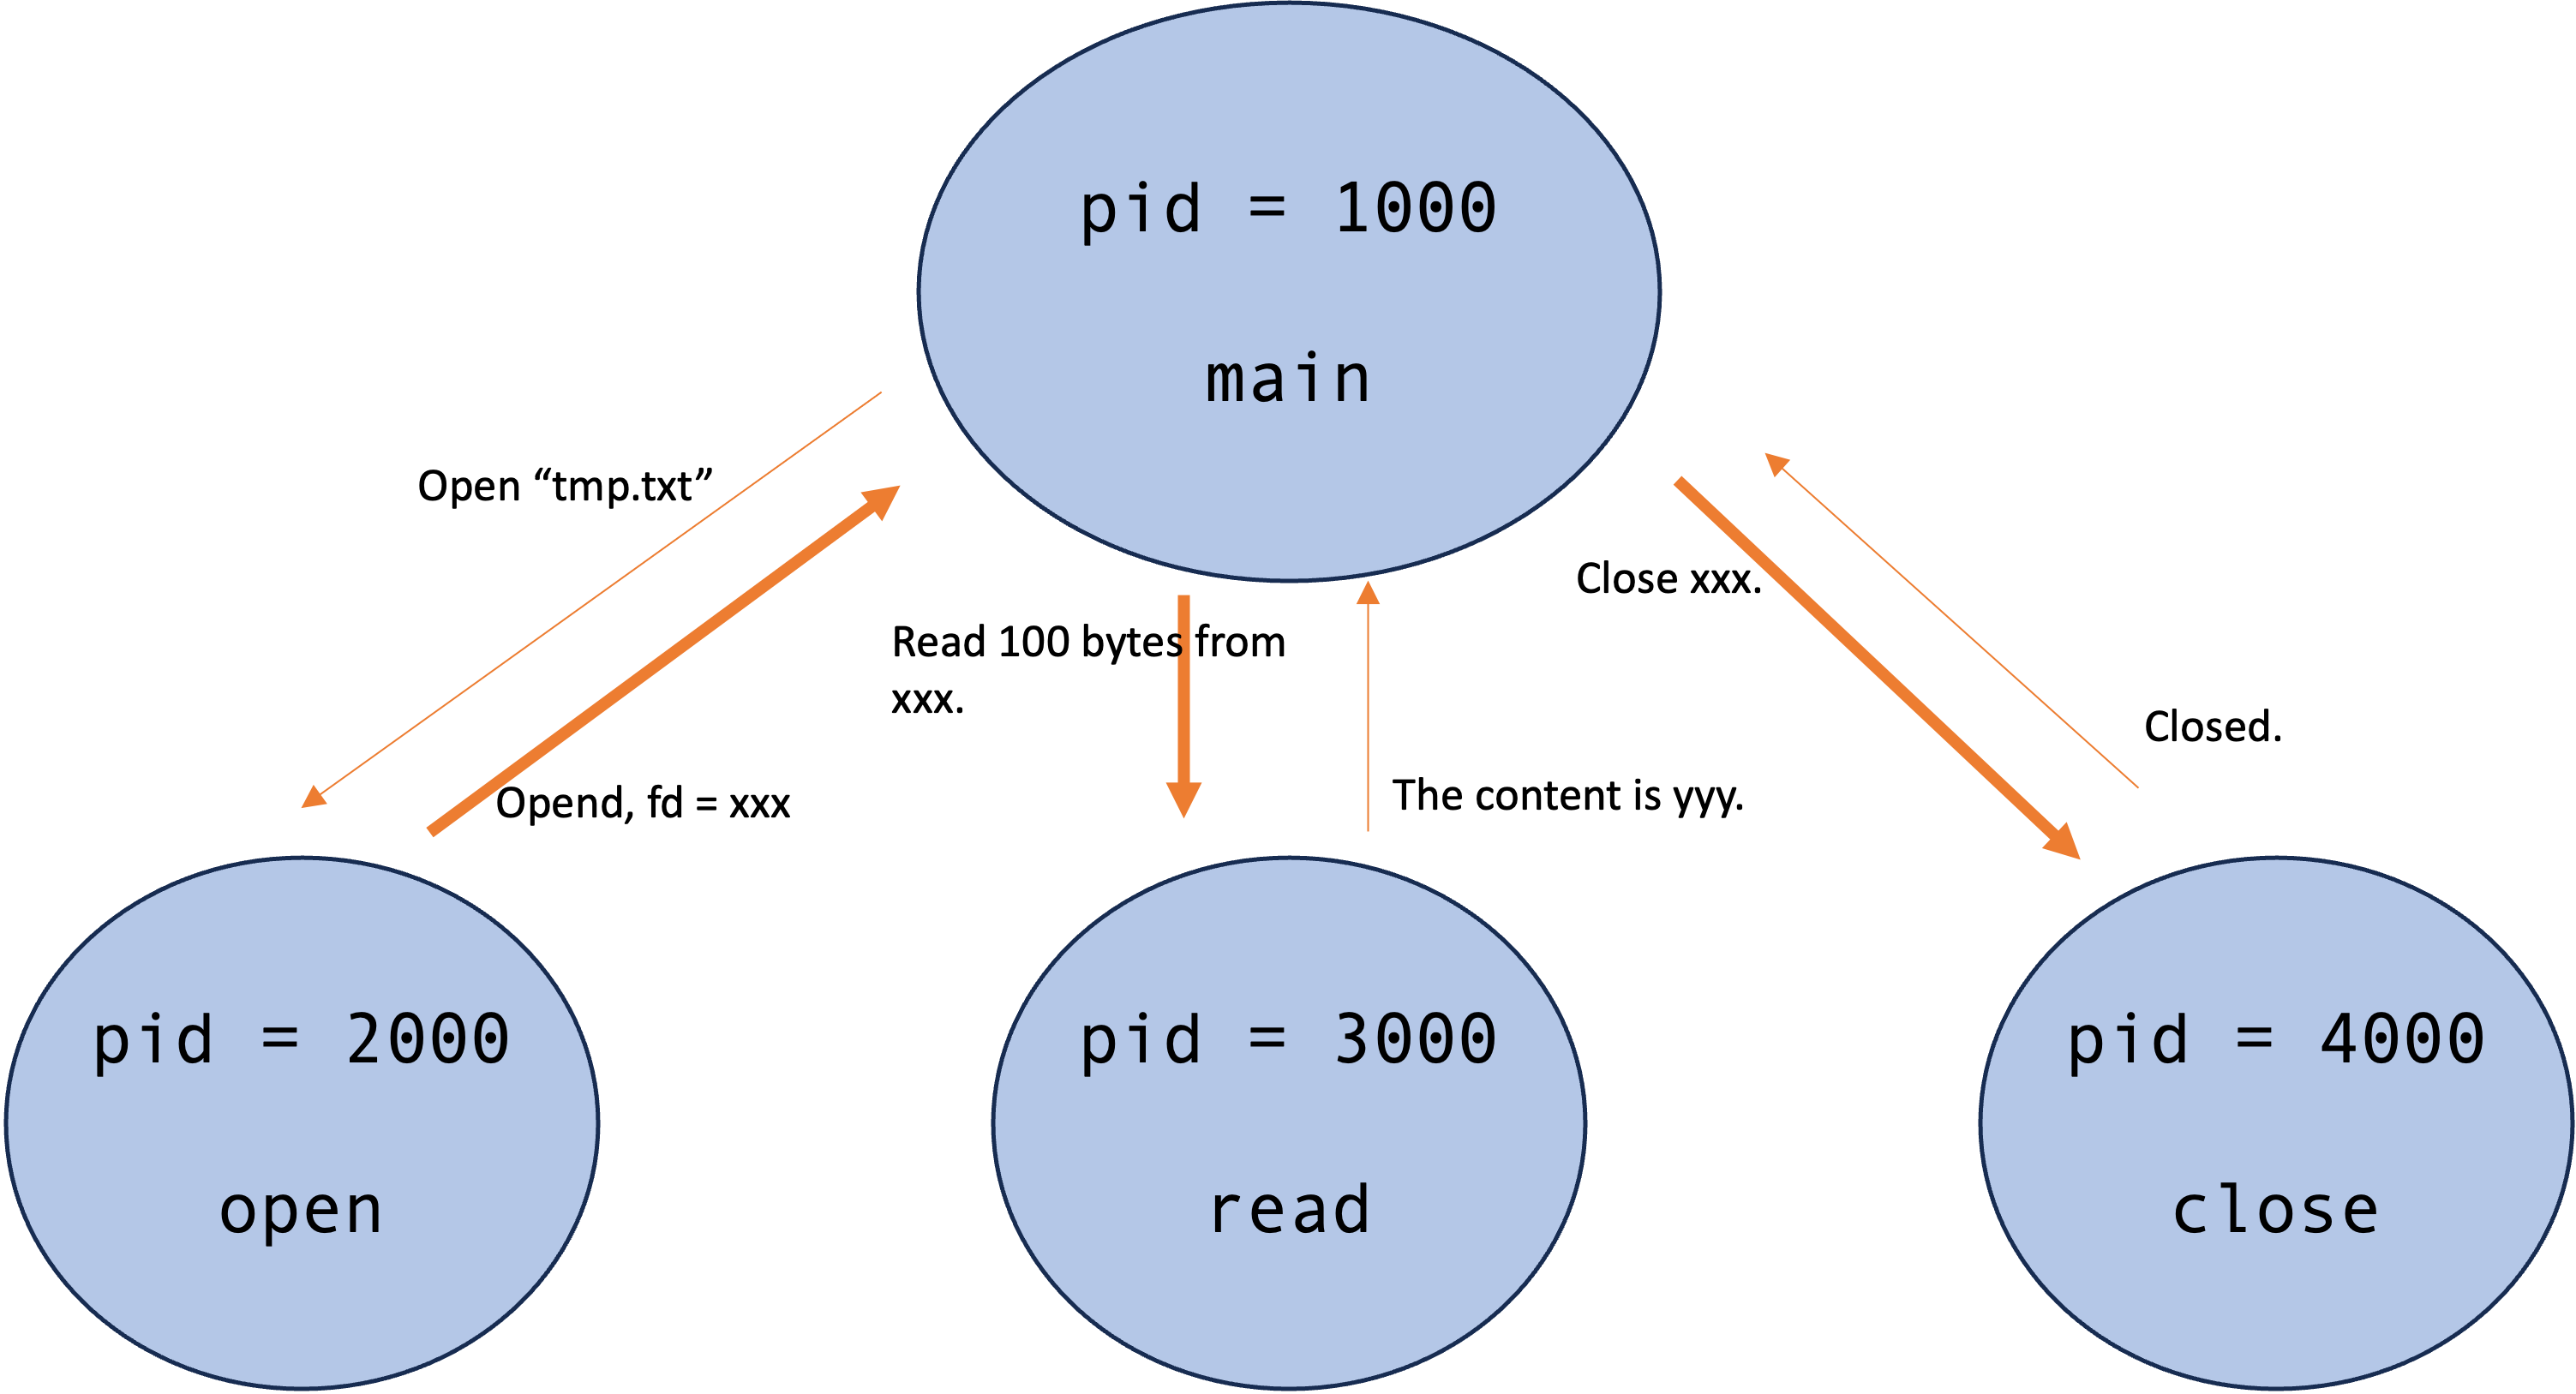
\includegraphics[width=1.8\columnwidth]{./img/fd_transfer.png}
  \end{center}
  \caption{Illustration of the concept of file descriptor transfer between shadow processes.
    The main process requests the shadow process to execute system calls, along with the required arguments.
    The thick arrows indicate the transfer of file descriptors over the control messages exchanged through IPC.}
  \label{img:fd-transfer}
\end{figure*}

\subsection{Design Overview}
The overview of proposed method is shown in \Fref{img:proposal-overview}.
\begin{figure}[t]
  \begin{center}
    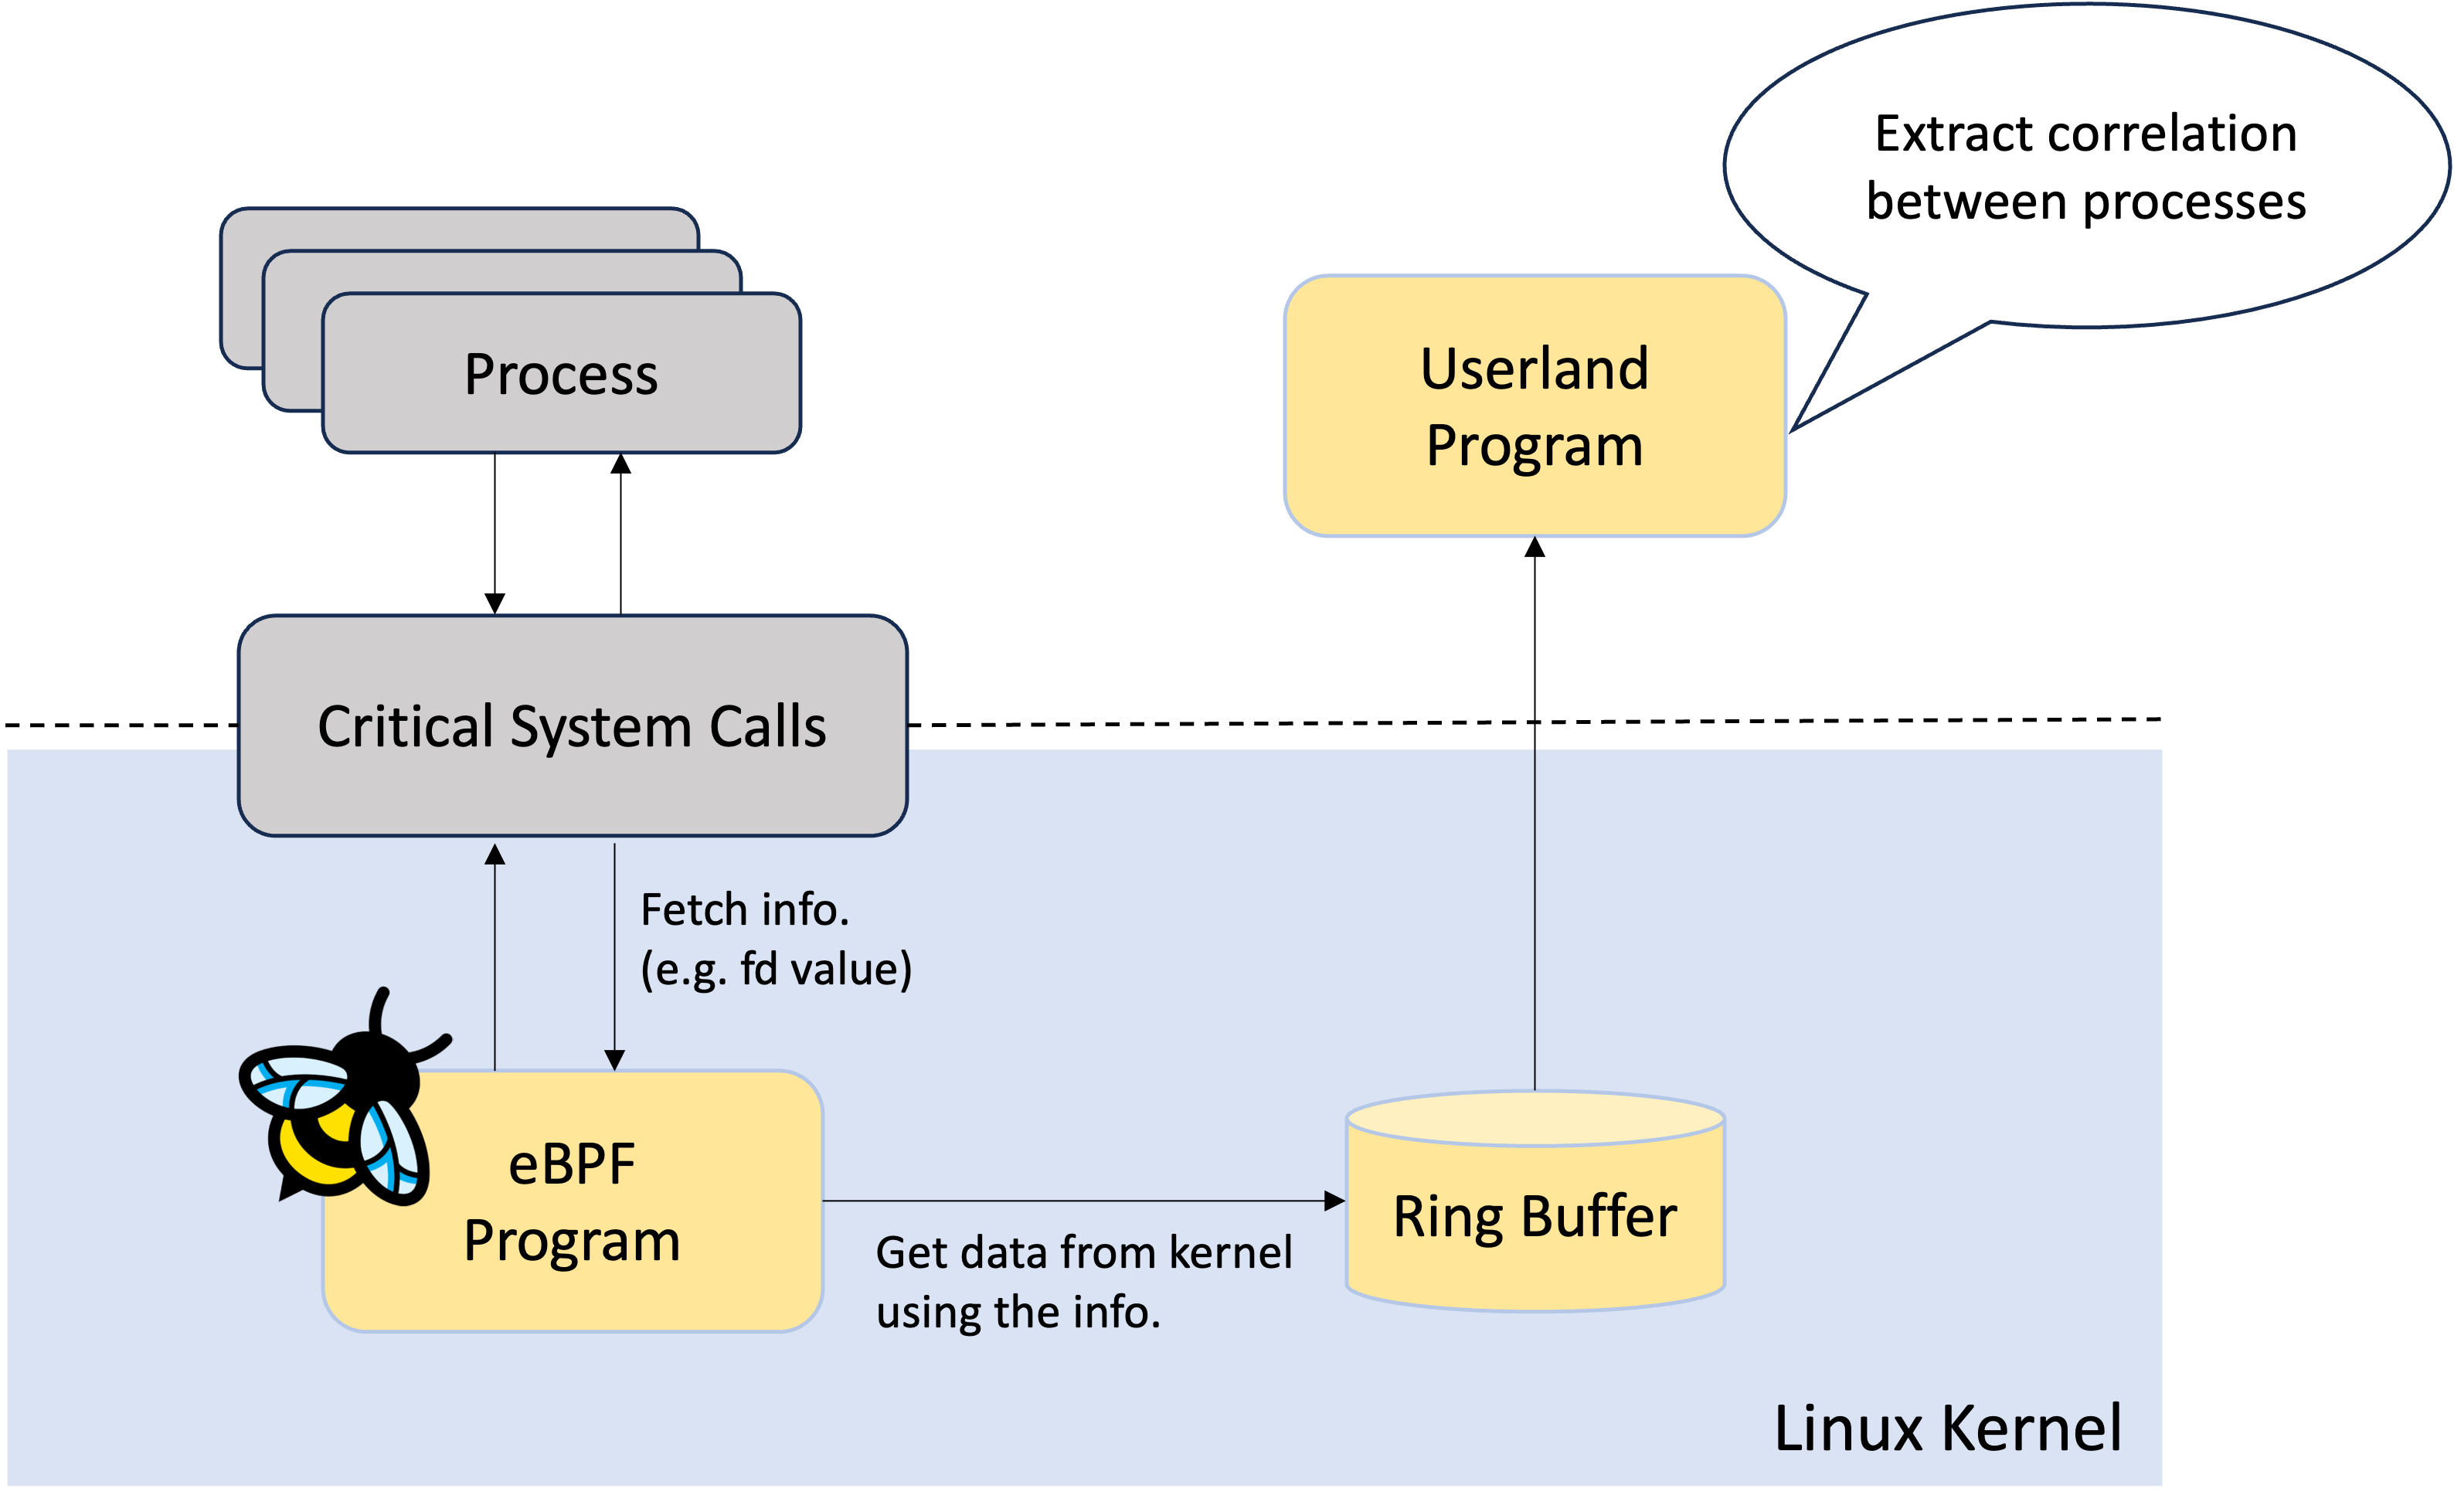
\includegraphics[width=\columnwidth]{./img/proposal_overview.png}
  \end{center}
  \caption{Illustration of the concept of file descriptor transfer between shadow processes.
    The main process requests the shadow process to execute system calls, along with the required arguments.
    The thick arrows indicate the transfer of file descriptors over the control messages exchanged through IPC.}
  \label{img:proposal-overview}
\end{figure}



\section{Experiment To Be Conducted}
\textbf{The experiment described in this section are still in the conceptual
  stage, but are planned to be conducted after the detail of implementation is fixed.}

\subsection{Performance Comparison with with User Space Implementation}
It could be achieved without inspecting kernel space to extract the correlation between processes.
For example, one solution was proposed in \cite{Weiqin:ShadowAttack} that
tracks changes to file descriptors in \texttt{/proc/fd} are recorded and subsequently analyzed
every timne a system call related to pipe, socket or file IO operation is executed as shown in \Fref{img:old-method}.
\begin{figure}[tp]
  \begin{center}
    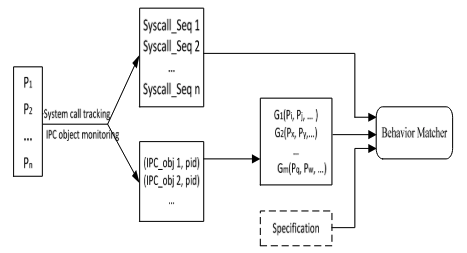
\includegraphics[width=\columnwidth]{./img/old_method.png}
  \end{center}
  \caption{Illustration of architecture of the countermeasure to shadow attacks proposed in
    \cite{Weiqin:ShadowAttack}.}
  \label{img:old-method}
\end{figure}
It should provide some insight about the efficiency of our method to compare the performance of it
with that of user space implementations.

We expect that our method will be more efficient than the user space implementations in the following reasons:
\begin{itemize}
  \item User space approach should confront the large overhead of copying data from kernel space to user space
        \cite{Weiqin:ShadowAttack,jia2023programmable}, but
        in our system that overhead will be mitigated with the efficient data sharing mechanism of eBPF maps.

  \item eBPF can filter out unnecessary information within kernel space before passing it to user space.
\end{itemize}

\subsubsection{Feasibility of Our Method}
We need to evaluate how accurately our method can detect the correlation between processes
while keeping false positive rate low.

For this purpose samples of shadow attack malware have to be prepared. In addition to that,
preparing specification malware detectors is required as the scope of this research is to
efficiently extract the correlation between processes.


\section{Conclusion}
In this paper, we highlighted the existence of shadow attacks,
which pose a significant threat by evading existing specification-based detectors.
To counter these attacks, we proposed a method leveraging eBPF to rapidly detect correlations
between shadow processes and discussed the detailed implementation of this approach.

Moving forward, our primary attention will be directed towards completing
the implementation specifics and carrying out the scheduled experiments to authenticate
our methodology in real-life situations.







\bibliographystyle{unsrt}
{
  \footnotesize
  \bibliography{bib, export}
}

\end{document}
